\subsection{Reference Height Temperature}

\subsubsection{Annual Mean Anomaly}

\begin{figure}[H]
	\centering
	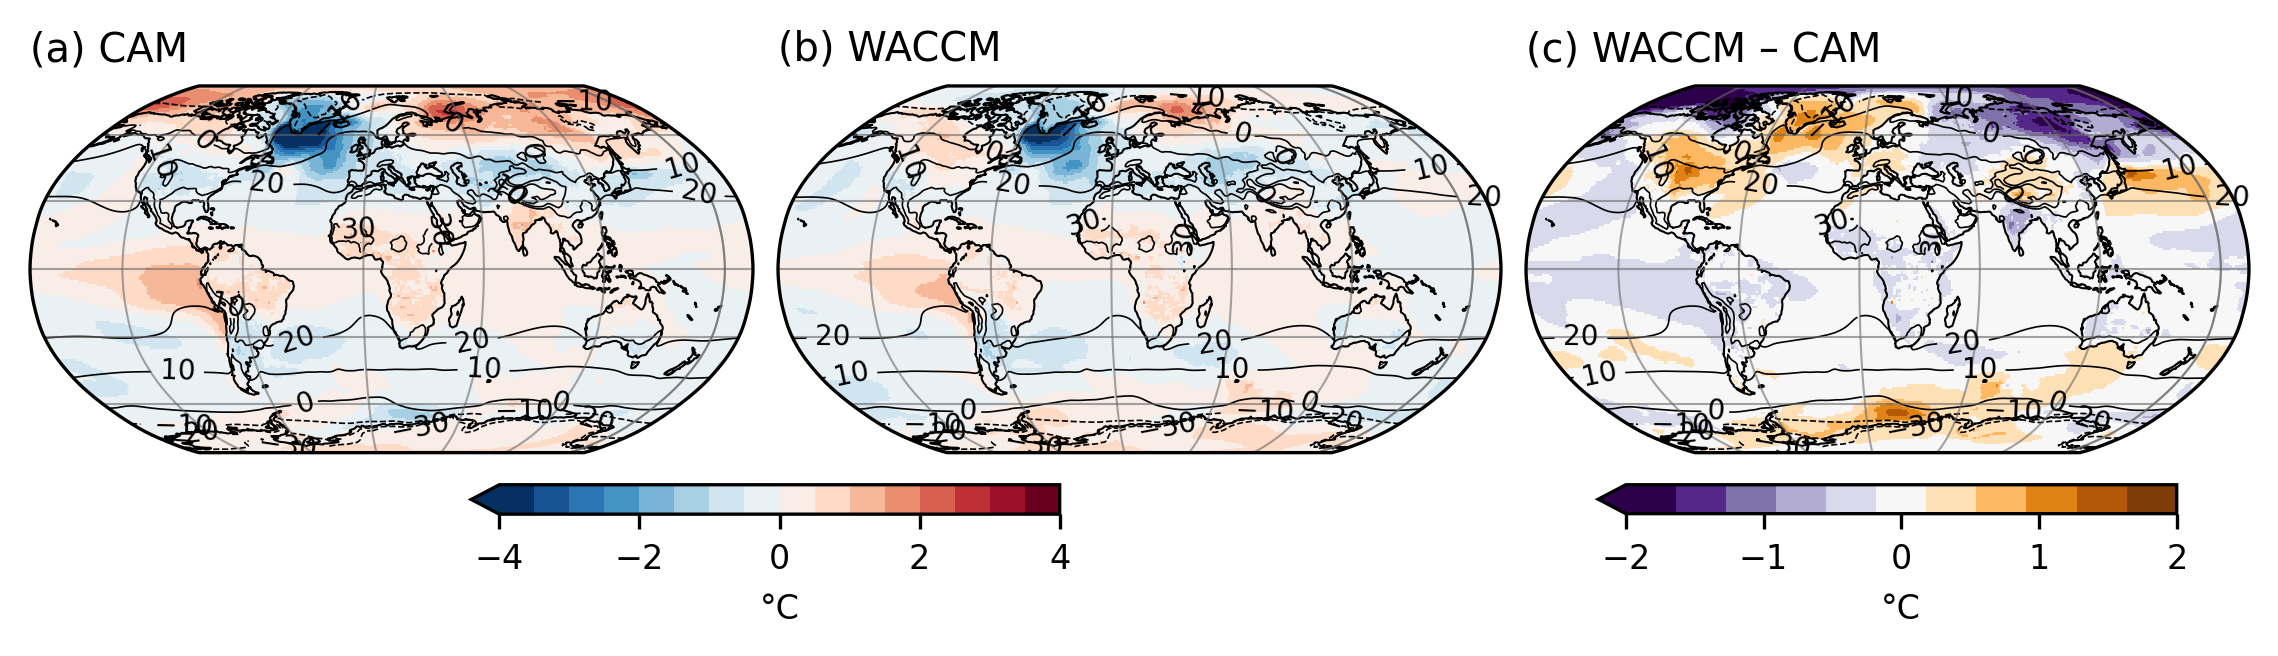
\includegraphics[width=\linewidth]{/Users/Simone/Documents/Uni/Master/Y2/Thesis/Paper_imgs/png/TREFHT_ann.png}
	\caption{Annual mean reference height temperature anomalies of 2080-2099 SAI2020 scenario compared to 2016-2035 Control scenario in (a) CAM and (b) WACCM. Difference between temperature anomalies shown in (c). 2016-2035 Control mean temperature shown in black contours in 10°C intervals.}
	\label{fig:TREFHT_ann}
\end{figure}

The annual mean reference height temperature anaomalies are shown in Figure \ref{fig:TREFHT_ann}, we learn:

\begin{itemize}
	\item Spatial patterns of warming and cooling generally similar, warming over equator (especially eastern Pacific), cooling in subtropics, warming over the poles.
	\item Warming hole over North Atlantic present in both models, due to AMOC collapse in POP2 ocean model used for both CESM2 simulations. 
	\item CAM shows clear warming in the Arctic ($>$1°C), slight warming in the Antarctic ($<$1°C)
	\item WACCM only shows significant warming over Barentsz sea ($>$1°C) and similar warming over the Antarctic compared to CAM.
	\item CAM warms more than WACCM in most of the Arctic, excluding Greenland. Tropics also experience slightly more warming in CAM.
	\item CAM cools more than WACCM in Greenland/North Atlantic, North America, Northwest Pacific and Southern Ocean South of Africa. Les clearly so on Tibetan Plateau.
\end{itemize}

TO DO:
\begin{itemize}
	\item extract maximum and minimum temperature anomalies
	\item Why: difference in warming hole intensity? natural variability? of andere background conditions/fresh water fluxes form atm model
	\item Check isobars
	\item Colorbar scale - witte 0 maar hoeveel levels verder? Super custom maken?
\end{itemize}



\subsubsection{JJA and DJF Seasonal Mean Anomaly}

\begin{figure}[H]
	\centering
	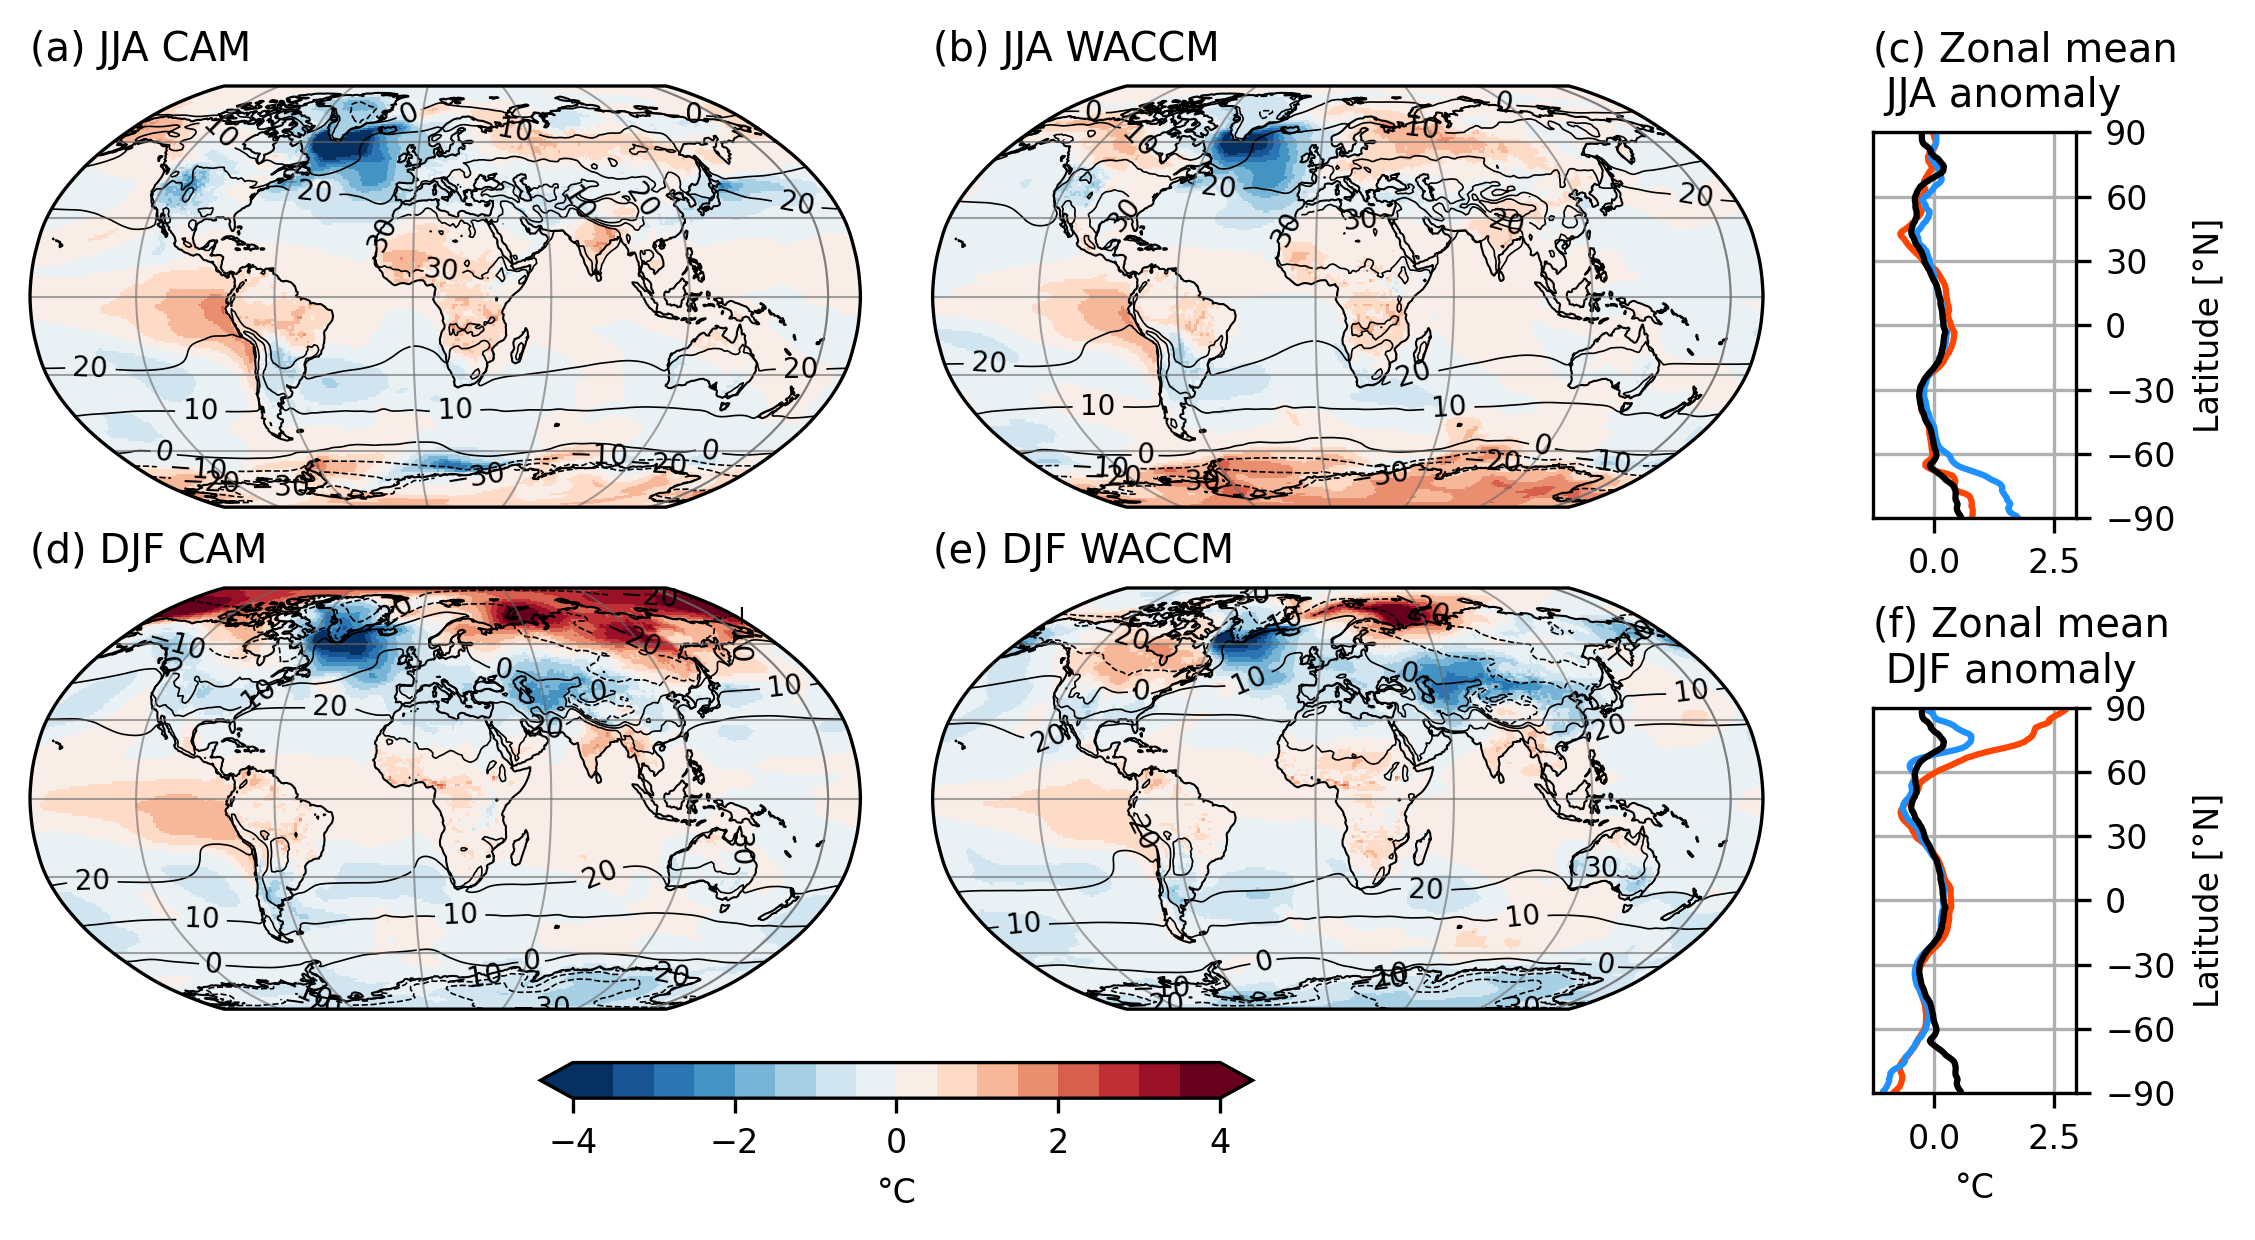
\includegraphics[width=\linewidth]{/Users/Simone/Documents/Uni/Master/Y2/Thesis/Paper_imgs/png/TREFHT_seas.png}
	\caption{JJA and DJF seasonal mean reference height temperature anomalies of 2080-2099 SAI2020 scenario compared to 2016-2035 control scenario in (a),(d) CAM and (b),(e) WACCM. 2016-2035 Control mean temperature shown in black contours in 10°C intervals. Zonal mean temperature anomalies shown in (c) and (f)}
	\label{fig:TREFHT_seas}
\end{figure}

The JJA and DJF seasonal mean reference height temperature anaomalies are shown in Figure \ref{fig:TREFHT_seas}, we learn:

\begin{itemize}
	\item In \textbf{JJA} the warming hole is the largest anomaly for both CAM and WACCM, showing slight differences in intensity but overall similar extent.
	\item WACCM shows significantly more warming than CAM over the whole of the Antarctic, also represented in the zonal mean anomaly. WACCM shows slightly more warming over Western Siberia and Norhtern Canada. 
	\item CAM shows more warming than WACCM over the Eastern Pacific, mainly showing warming over an much larger extent. CAM shows slightly more warming over Alaska, Western Africa and South Asia. 
	\item in \textbf{DJF} the warming hole is still present in both CAM and WACCM, again larger extent and more intense in CAM. 
	\item WACCM shows slightly more warming than CAM in the interior of Canada/Hudson Bay and slightly more cooling over Central Asia. 
	\item CAM shows much more warming of the Arctic and Eastern Siberia than WACCM, also represented in the zonal mean anomaly. CAM shows slightly more warming over the Eastern Pacific again, as it does in JJA.
\end{itemize}

TO DO:
\begin{itemize}
	\item figure out legend for line plot.
	\item Why: much more warming over Antarctic in WACCM? Possibly ozone hole, other dynamics? 20 jaar voor 2080 ook plotten om te kijken naar natural variability.
	\item Why: warming of Eastern Pacific, due to known behaviour of ITCZ in CAM?
	\item THESIS: interannual variability meer onderzoeken voor Arctic.
\end{itemize}


\subsubsection{Annual vs. Seasonal}
When comparing Figures \ref{fig:TREFHT_ann} and \ref{fig:TREFHT_seas} we learn:

\begin{itemize}
	\item Most of the differences observed between WACCM and CAM are attributable to the winter months in the respective hemispheres. 
	\item Overall the patterns observed in the anomalies are similar, most significant differences are observed in the Arctic and Antarctic. 
	\item annual en JJA DJF samenvoegen
	\item zonal mean anomaly WACCM en CAM bundelen
\end{itemize}